\chapter{Experimental evaluation} \label{sec:experimentsoutside}
The simulations conducted in the previous chapter form the basis for real world measurements and experimental evaluation of the MP-SRP-PHAT algorithm, and to test its performance and robustness in various conditions. In order to test the algorithm under ideal, controlled conditions, anechoic measurements were conducted. After that a series of outdoor sources and environments were tested. This chapter contains the results of the experiments. 

\section{Microphone array and acquisition system}
The equipment used for the experiments are listed below.
\begin{table}[!ht]
    \centering
	\begin{tabular}{ll} \toprule
	{Item \#}	&	{Description}\\
	    \bottomrule 
	        &   \textbf{{General}}                                       \\
	    1   &   4 B\&K  Type 4935 microphones                            \\
	    2   &   1 B\&K Module Type 3050-A-060 interface module           \\
	    3   &   Prototype tetrahedral microphone stand                   \\
		4   &   Relevant cables and wires                                \\
		5   &   PC with MATLAB, Python and B\&K Pulse software           \\
		\bottomrule 
            &  \textbf{{Anechoic measurements}}                           \\
		6	&   1 B\&K OmniPower loudspeaker                              \\
		7   &   2 custom spherical speakers                               \\
		8   &   1 Pioneer A-656 amplifier                                 \\
		9   &   1 B\&K Type 2270 hand-held analyzer                       \\
		\bottomrule 
		    &   \textbf{{Outdoor measurements}}                           \\
		10  &   1 B\&K Module Type 2831 battery module                    \\
		11  &   4 B\&K microphone ellipsoidal windscreens                  \\
		\bottomrule 
	\end{tabular}
\end{table}

A prototype microphone array was used to record sound sources. The array contains 4 B\&K Type 4935 microphones placed in a tetrahedral configuration (Fig. \ref{fig:arraymic1}). 

The height of the array can be adjusted by translating the middle vertical rod, which is placed on a tripod. The microphone array allows adjustment of the array aperture size between 10cm-1m. The 4 microphones are omni-directional and mounted on the array vertically (pointing upwards). 
\begin{wrapfigure}{r}{0.35\textwidth}
    \centering
    \includegraphics[width=0.4\textwidth]{Figures/Arraymicrophone.png}
    \caption{\label{fig:arraymic1}Prototype tetrahedral array used for measurements}
\end{wrapfigure}
B\&K Pulse software suite was used for recording. B\&K Module Type 3050-A-060 was used as the main interface sound card and microphones were plugged into it with BNC connectors. During outside measurements, foam microphone windscreens were mounted on the microphones and a B\&K battery module was used to power the soundcard. The recordings are all 16bit .wav files, recorded with a sampling rate of 131072Hz (the maximum sampling rate available on the system). Two different values of the tetrahedral array aperture are used, 1m and 39.5cm, resulting in two different sizes for the tetrahedral array, large and small. For the large tetrahedral array, the microphones are placed at $M_1(x,y,z)=(0.5, 0, 0)$, $M_2(x,y,z)=(-0.5, 0, 0)$, $M_3(x,y,z)=(0, -0.866, 0)$ and $M_4(x,y,z)=(0, -0.433, 0.7071)$. For the small tetrahedral the locations are  $M_1(x,y,z)=(0.1975, 0, 0)$, $M_2(x,y,z)=(-0.1975, 0, 0)$, $M_3(x,y,z)=(0, -0.3421, 0)$ and $M_4(x,y,z)=(0, -0.171, 0.2793)$.


\section{Anechoic Measurements}
\subsection{Localizing a single sound source}




%\begin{figure}[H]
%    \centering
%    \includegraphics[width=0.5\textwidth]{Figures/Arraymicrophone.png}
%    \caption{Prototype microphone array}
%    \label{fig:micarraypic}
%\end{figure}

\begin{figure}[H]
    \centering
    \includegraphics[width=0.8\textwidth]{Figures/Anechoicexp1.png}
    \caption{Sketch of the experiment}
    \label{fig:Anechoic1}
\end{figure}

Sounds from a single loudspeaker were recorded with the array. The source was a B\&K Omnisource Type 4296 with operating frequency of 100Hz-5kHz. The loudspeaker position was fixed and the microphone array was rotated around its axis in order to change the relative source location (azimuth). The setup is described by Fig. \ref{fig:Anechoic1} where the two point source positions are shown: (90$\degree$,0$0\degree$) and (30$\degree$,0$\degree$). The loudspeaker played pink noise\footnote{A recording of 300Hz sinusoidal wave was also performed to display the delays between the microphones. The results can be seen in Appendix. \ref{add_Meas_1}}. In order to recreate far-field conditions and to approximate plane wave propagation, in the limited space of the anechoic chamber, the array was placed as far away from the source as possible and also the array aperture was reduced to 0.395m. Temperature of the lab was 22 $\degree$C.



\subsubsection{Results}
The energy maps of the SRP-PHAT and minimum power SRP-PHAT algorithms are computed and displayed in Fig. \ref{fig:1srcAnechoic}
\begin{figure}[H]
    \centering
    \begin{subfigure}[b]{0.96\textwidth}
    \centering
    \includegraphics[width=0.95\textwidth]{Figures/Anechoic0Deg1SrcNorm.png}
\end{subfigure}
\vskip \baselineskip
\begin{subfigure}[b]{0.96\textwidth}
    \centering
    \includegraphics[width=0.95\textwidth]{Figures/Anechoic0Deg1SrcMinPow.png}
\end{subfigure}
\caption{Figures depict SRP-PHAT (top) and minimum power SRP-PHAT (bottom) localization for source around (90 $\degree$, 0$\degree$) in an anechoic Room}
\label{fig:1srcAnechoic}
\end{figure}
The source was localized slightly above 0$\degree$ elevation. This is because the top microphone of the array was on the same horizontal axis as the acoustic center of the sound source. 
%This shift can also be explained by the inaccuracies in the microphone positions on the microphone array. The prototype microphone array allows the 3 microphones on the horizontal axis to move up and down in order to adjust the microphone array aperture relative to the "fixed" top microphone. Therefore there might be a maladjustment in the position of the 3 lower microphones relative to the top microphone thus creating an incorrect position on the vertical axis and ultimately an error in the localization. 
The height of the microphone array was later increased in order to place the 3 lower microphones on the same vertical axis as the acoustic center of the sound source. The following figure shows the results for source at (30 $\degree$, 0$\degree$). 
%This could also be due to a tilt of the array or the source not being in the far-field.
%As will be seen in the following graphs of the sound source at 30 $\degree$ azimuth the elevation error is reduced. No further investigation are done. 
\begin{figure}[H]
    \centering
    \begin{subfigure}[b]{0.96\textwidth}
    \centering
    \includegraphics[width=0.95\textwidth]{Figures/Anechoic30Deg1SrcNorm.png}
\end{subfigure}
\vskip \baselineskip
\begin{subfigure}[b]{0.96\textwidth}
    \centering
    \includegraphics[width=0.95\textwidth]{Figures/Anechoic30Deg1SrcMinPow.png}
\end{subfigure}
\caption{Figures depict from top-to-bottom SRP-PHAT and minimum power SRP-PHAT localization for source at (30$\degree$,0$\degree$) in an anechoic room}
\end{figure}
\subsection{Localizing 2 sources and computing their relative level difference}
It is not enough to simply localize the outdoor sound sources. The level of the sound source is important as well. Since, PHAT algorithm inherently normalizes the input signal, only relative level difference can be directly retrieved (It will be shown later how absolute levels can be retrieved once the relative levels are correctly computed). This experiment was run in the anechoic chamber with focus on retrieving the relative sound level difference of two sources playing at the same time.  Two custom spherical speakers were used to play the source signal and the aperture size of the array was set at 0.395m. One source placed at (90$\degree$, 0$\degree$) played pink noise at 46dBA, the second source placed at (130$\degree$, 0$\degree$) played uncorrelated pink noise at 52dbA. The low frequencies (<200Hz) were filtered out in order to accommodate for the speaker used. The sound from each speaker was measured individually using a level meter in order to check the playback levels. Temperature of the room was recorded at 22$\degree$C.
\begin{figure}[H]
    \centering
    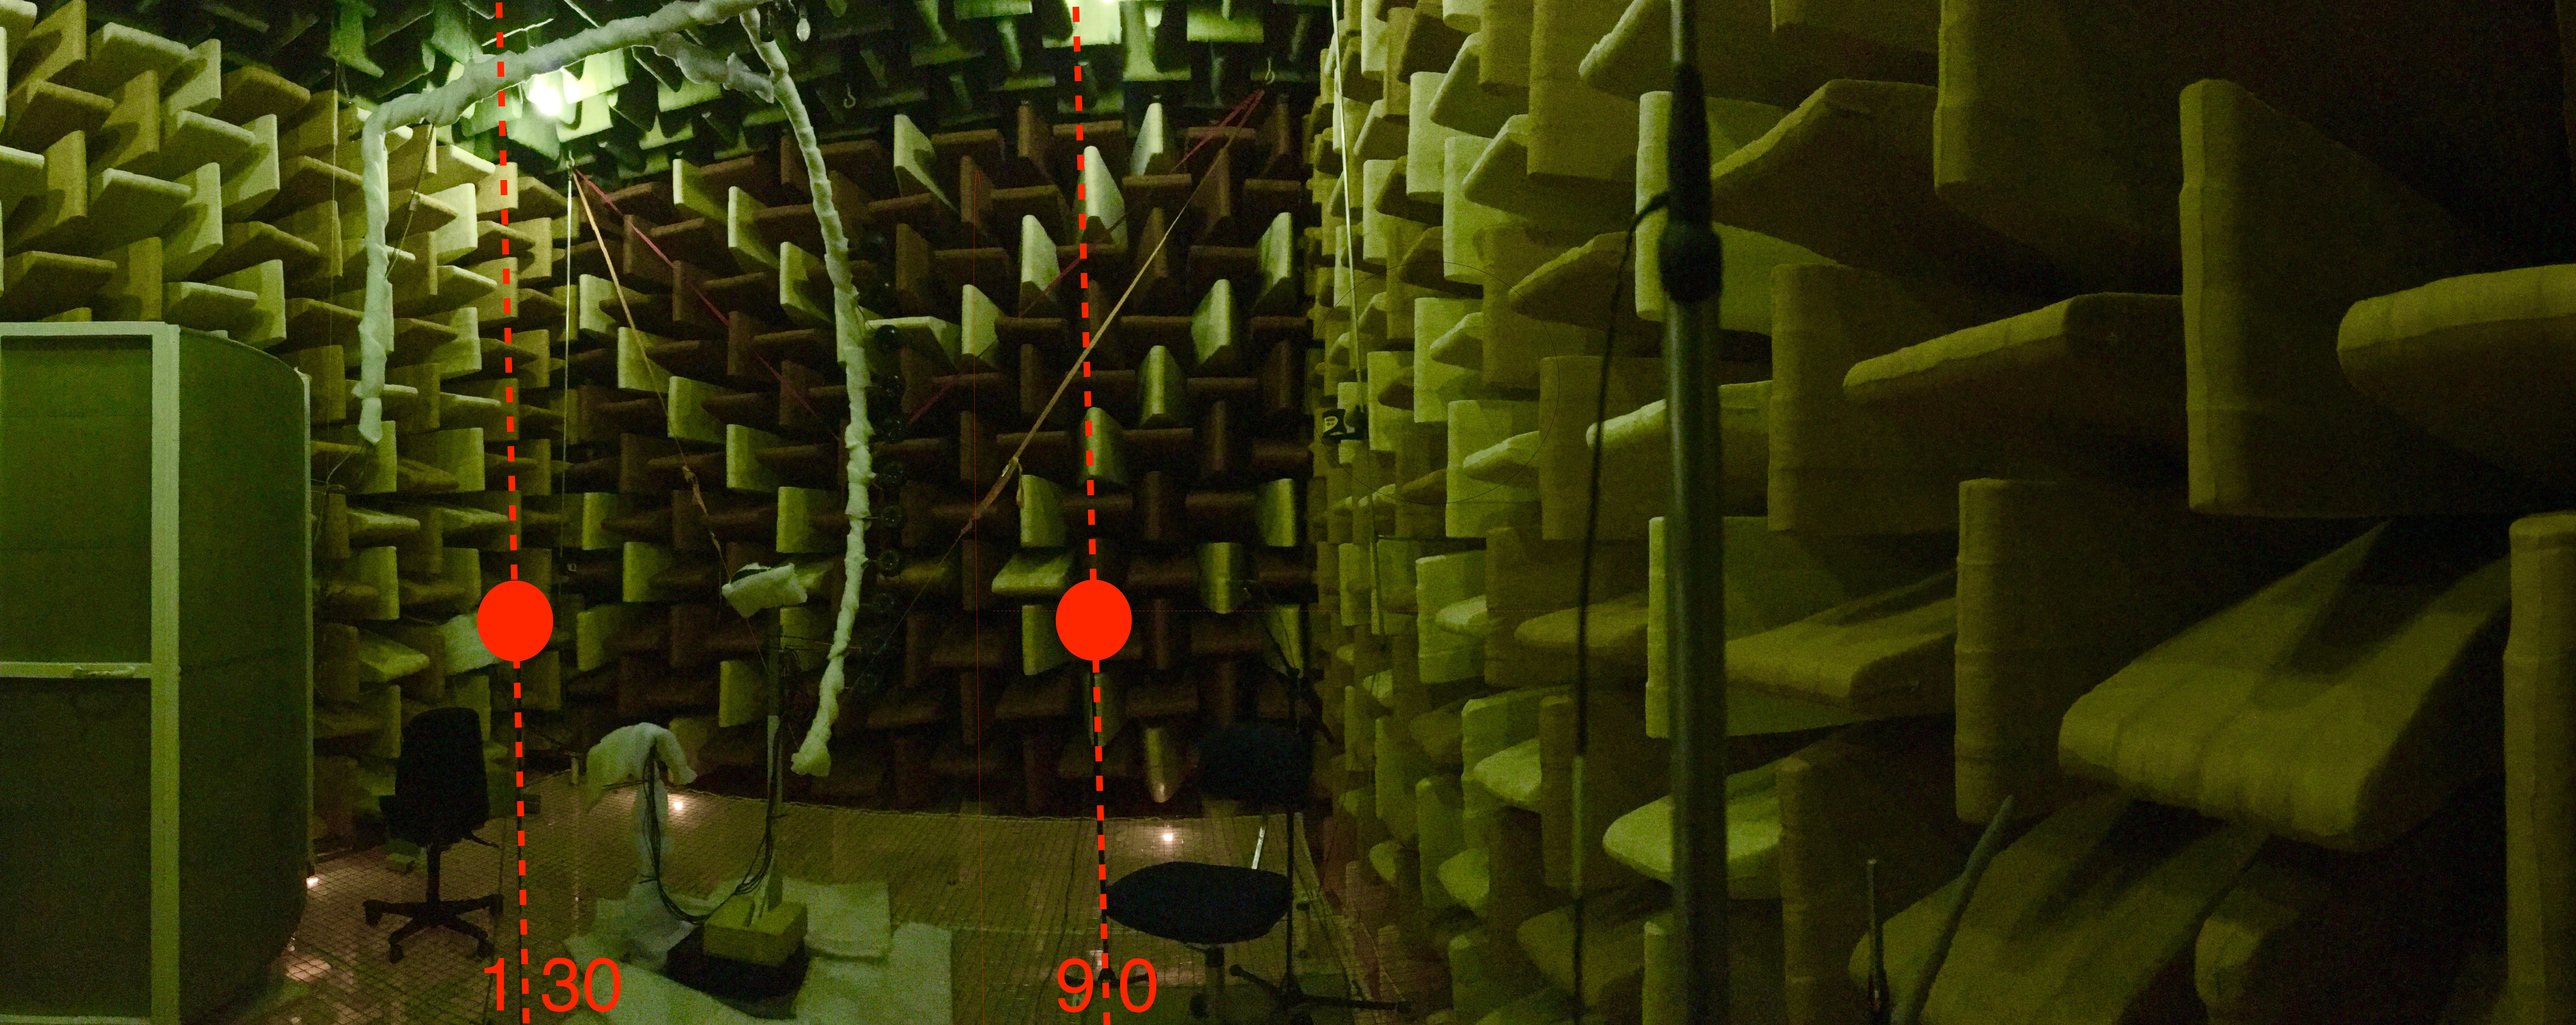
\includegraphics[width=1\textwidth]{Figures/AnechoicPic.jpg}
    \caption{Picture of the set up. The anechoic chamber was filled with misc. equipment, therefore the sources have been replaced by red dots for clarity. 90$\degree$ and 130$\degree$ azimuth are also drawn on top of the picture.}
    \label{fig:Anechoicpic1}
\end{figure}
\begin{figure}[H]
    \centering
    \includegraphics[width=0.7\textwidth]{Figures/Anechoicexp3.png}
    \caption{Diagram of the experiment}
    \label{fig:Anechoicexp3}
\end{figure}
\subsubsection{Results}
\begin{figure}[H]
    \centering
    \begin{subfigure}[b]{0.96\textwidth}
    \centering
    \includegraphics[width=0.95\textwidth]{Figures/Anechoic2SrcNorm.png}
\end{subfigure}
\vskip \baselineskip
\begin{subfigure}[b]{0.96\textwidth}
    \centering
    \includegraphics[width=0.95\textwidth]{Figures/Anechoic2SrcMinPow.png}
\end{subfigure}
\caption{Figures depict from top-to-bottom SRP-PHAT and minimum power SRP-PHAT localization}
\end{figure}
During the experiment, the anechoic chamber was not completely empty and some reflections can be observed at and below 12dB dynamic range, which potentially masks the secondary (lower magnitude) source. Also, since the speakers were relatively close to the array, the cone approximation has larger errors. This can reduce the size of overlap of the multiple cones from the various microphones. This can be seen in the result for normal SRP-PHAT here, where the cones for the secondary cones barely overlap. Applying minimum power SRP-PHAT can then completely hide the secondary source. For this measurement however, the secondary source can just be seen. The results from normal SRP-PHAT showed the secondary source level to be playing at -6.81dB relative to the main source. Understandably, due to the issues discussed here, the results from the minimum-power showed the secondary source level to be -8.18dB relative to the main source. Both normal and min power localized the peak of the main sound source at the same location (130$\degree$,-1$\degree$). However, the peak of the secondary source was localized at (95$\degree$,-2$\degree$) by normal SRP-PHAT and at (94$\degree$,-1$\degree$) by min power SRP-PHAT. This minor difference can be attributed to the fact that the peak at (95$\degree$,-2$\degree$) was removed by the minimum power algorithm. The total power received at $M_1$ for the delay associated with the peak location was calculated according to Section \ref{srcLvlRetrieval}. It was computed to be 50.57dB.

%The maximum dynamic range achievable is correlated to the amount of reflections and noise in the environment, specially when localizing multiple sources. 
%For near free-field conditions with few reflections a dynamic range of 12dB can be achieved whereas very reflective environments will limit the dynamic range to 3dB in the worst case.
%
%\begin{figure}[H]
%    \centering
%    \begin{subfigure}[t]{0.5\textwidth}
%    \centering
%    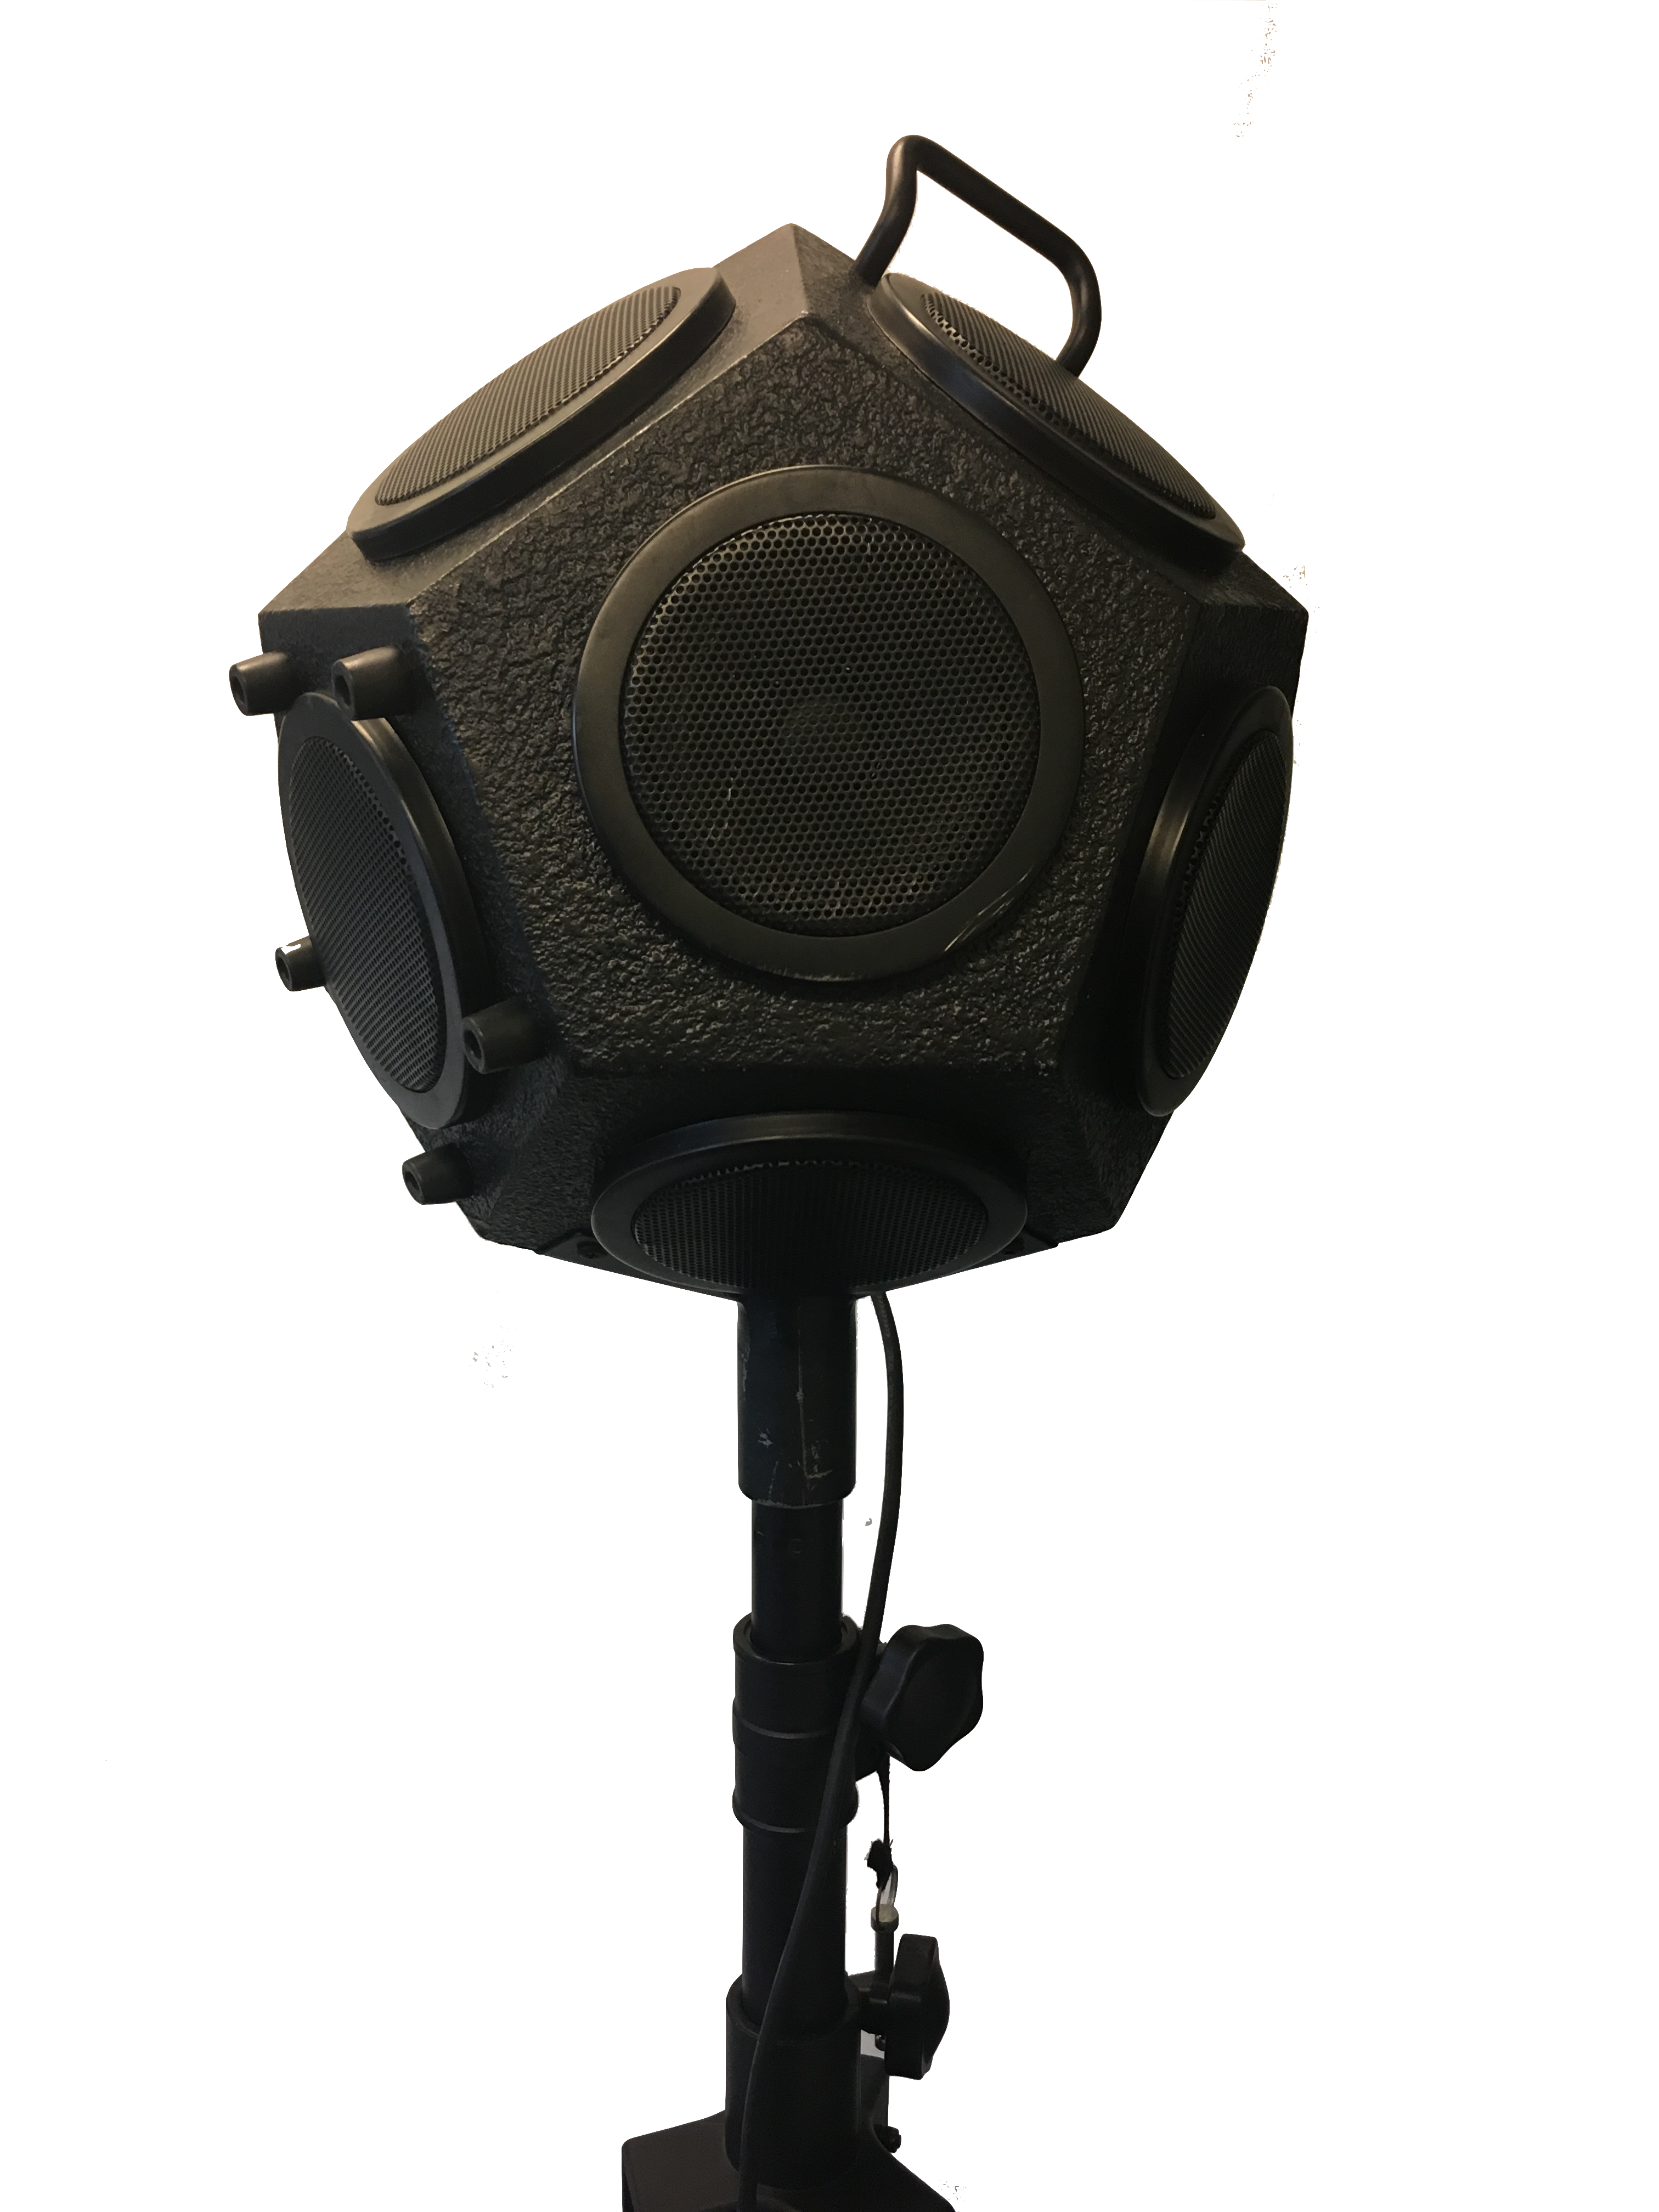
\includegraphics[width=0.9\textwidth]{Figures/IMG_7337.png}
%    \caption{B\&K Omnisource}
%    \label{fig:Omnisource}
%\end{subfigure}%
%\begin{subfigure}[t]{0.5\textwidth}
%        \centering
%    \includegraphics[width=0.9\textwidth]{Figures/Arraymicrophone.png}
%    \caption{Prototyped microphone array}
%    \label{fig:Array}
%\end{subfigure}
%\end{figure} 
\section{Outdoor measurements}
In order to test the algorithm in real conditions, several outdoor measurements in various conditions were conducted. Experiments were run in a construction field, in outdoor and indoor concerts, in traffic and in a chalk mining field. The recordings are again done at the maximum sample rate available in the system, viz, 131072Hz. The microphone array aperture unless otherwise mentioned, was set at 1m, since the sources were always sufficiently far away. Photos of the measured outdoor environment were taken using a camera having a known angle of view, such that the azimuth and elevation of the photos was known. Finally, the localization results were overlaid on the photos.
\subsection{Single static source on a construction field}
In this experiment, a single construction machine working in a fixed position was recorded by the microphone array. The source was more than 20 meters away. Fig. \ref{fig:Scenario1pic} describes the setup. The measurement system was set in the middle of a road, outside the construction field. There was a big office building with a smooth faćade behind the setup. Temperature was recorded at 23$\degree$C, speed of wind was 2m/s from (180$\degree$, 0$\degree$). Fig. \ref{Fig:OutdoorLast1Src} displays the results.
\begin{figure}[H]
    \centering
    \begin{subfigure}[b]{1\textwidth}
    \includegraphics[width=1\textwidth]{Figures/Scenario1pic.jpg}
    \end{subfigure}
    \vskip \baselineskip
    \begin{subfigure}[b]{0.8\textwidth}
    \centering
    \includegraphics[width=0.8\textwidth]{Figures/scenario2diagram.png}
    \centering
    \end{subfigure}
    \caption{Figure shows the picture of the construction field (top) and the top view schematic of the construction field (bottom)}
    \label{fig:Scenario1pic}
\end{figure}
\subsubsection{Results}
\begin{figure}[H]
    \centering
    \begin{subfigure}[b]{0.96\textwidth}
    \centering
    \includegraphics[width=0.95\textwidth]{Figures/OutsideLastNorm.png}
\end{subfigure}
\vskip \baselineskip
\begin{subfigure}[b]{0.96\textwidth}
    \centering
    \includegraphics[width=0.95\textwidth]{Figures/OutsideLastMinPow.png}
\end{subfigure}
\caption{Figures depict from top-to-bottom SRP-PHAT and minimum power SRP-PHAT localization}
\label{Fig:OutdoorLast1Src}
\end{figure}
The recordings were made 51sec long (the duration during which the machine was in the same position). Since the recordings used to localize are of a relatively long duration, short-timed or spontaneous sound events would not appear on the map, since they are effectively averaged out by the GCC-PHAT algorithm. The results are shown in figure \ref{Fig:overlayimageoutside2}. Even though the machine itself did not move, the excavator arm moved around the body of the machine emitting noise as it excavated. As can be seen, the sounds emitted at different positions around the motor due to the arm do not appear on the result image. The dynamic range of the map has been adjusted to filter out the reflections and less powerful sources. Results for dynamic range of 12dB and 6dB are shown. It is indeed difficult to get a clean map for a large dynamic range, as more and more reflections from the source become apparent, as well as other distant sources in the construction field and their own reflections. In addition, other noise sources such as the wind noise or other diffuse reflections can appear on the results.
\begin{figure}[!ht]
    \centering
    \begin{subfigure}[b]{0.96\textwidth}
    \centering
    \includegraphics[width=1\textwidth]{Figures/Outside2MinPow12dB.png}
\end{subfigure}
\vskip \baselineskip
\begin{subfigure}[b]{0.96\textwidth}
    \centering
    \includegraphics[width=1\textwidth]{Figures/Outside2MinPow6dB.png}
\end{subfigure}
\caption{Figures depict localization results overlaid on the photo of the measured source with dynamic range of 12dB (top) and 6dB (bottom)}
\label{Fig:overlayimageoutside2}
\end{figure}
\subsection{3 static sources on a construction field}
In this experiment, 3 distinct noise sources were measured: a tapping machine in a hole in the ground located at (180$\degree$,<0$\degree$) and two excavators located between (120$\degree$-150$\degree$,0$\degree$). Fig. \ref{fig:Scenario2} describes the setup. Fig. \ref{Fig:Outdoorpicfull} displays the results.
\begin{figure}[H]
    \centering
    \begin{subfigure}[b]{0.96\textwidth}
    \includegraphics[width=1\textwidth]{Figures/scenario3pic.jpg}
    \end{subfigure}
    \vskip \baselineskip
    \begin{subfigure}[b]{0.96\textwidth}
    \centering
    \includegraphics[width=1\textwidth]{Figures/scenario1diagram.png}
    \end{subfigure}
    \caption{Panorama of the construction field at the center point of the microphone array (top) and Top view schematic of the construction field (bottom)}
    \label{fig:Scenario2}
\end{figure}
\subsubsection{Results}
\begin{figure}[H]
    \centering
    \begin{subfigure}[b]{1\textwidth}
    \centering
     \includegraphics[width=1\textwidth]{Figures/Scenario1DYN6.png}
\end{subfigure}
\vskip \baselineskip
\begin{subfigure}[b]{1\textwidth}
    \centering
    \includegraphics[width=1\textwidth]{Figures/Scenario1DYN3.png}
\end{subfigure}
\caption{Figures depict from top-to-bottom Min SRP-PHAT with dynamic range of 6dB and 3dB}
\label{Fig:Outdoorpicfull}
\end{figure}
\begin{figure}[H]
\vskip \baselineskip
\begin{subfigure}[b]{1\textwidth}
    \centering
    \includegraphics[width=0.9\textwidth]{Figures/Scenario1DYN3Zoomed.png}
\end{subfigure}
\caption{Zoomed figure depict from top-to-bottom Min SRP-PHAT with dynamic range of 3 dB}
\label{Fig:Outdoorpicfull}
\end{figure}
\subsection{Sport event with crowd and PA system }
Measurements were performed during a sport competition outside, two main noise sources are present. The first one was a distributed PA system that covers all the zone as shown in figure \ref{fig:Scenario1diagram}, the second one was a crowd at (0°,0°), however the crowd level was quite low compared to the music level.
\begin{figure}[H]
    \centering
    \includegraphics[width=1\textwidth]{Figures/bmxracepic.jpg}
    \caption{Panorama of the setup at the center point of the microphone array}
    \label{fig:Scenario3}
\end{figure}
\begin{figure}[H]
    \centering
    \includegraphics[width=0.8\textwidth]{Figures/bmxrace1.png}
    \caption{Top view of the scenario}
    \label{fig:Scenario1diagram}
\end{figure}
\subsubsection{Results}
\begin{figure}[H]
    \centering
    \begin{subfigure}[b]{1\textwidth}
    \centering
    \includegraphics[width=1\textwidth]{Figures/BMX_1_6.png}
\end{subfigure}
\vskip \baselineskip
\begin{subfigure}[b]{1\textwidth}
    \centering
    \includegraphics[width=1\textwidth]{Figures/BMX_1_3.png}
\end{subfigure}
\caption{Figures depict from top-to-bottom Min SRP-PHAT with dynamic range of 6dB and 3dB}
\label{Fig:bmxracedyn}
\end{figure}
\begin{figure}[H]
    \centering
    \begin{subfigure}[b]{1\textwidth}
    \centering
    \includegraphics[width=1\textwidth]{Figures/BMX_1_6_zoomed.png}
\end{subfigure}
\vskip \baselineskip
\begin{subfigure}[b]{1\textwidth}
    \centering
    \includegraphics[width=1\textwidth]{Figures/BMX_1_3_zoomed.png}
\end{subfigure}
\caption{Figures depict from top-to-bottom Min SRP-PHAT with dynamic range of 6dB and 3dB}
\label{Fig:bmxracezomm}
\end{figure}
As can be seen the results are not good. Based on these results, the localization performance of the algorithm was simulated when multiple sources were playing the same sound (Sec. \ref{sec:Coherent}). It was found that when multiple coherent sources are present, the algorithm can fail as the constant phase difference between the multiple sources can be detected as a pseudo-source. 
\subsection{Outdoor concert}
Measurements were performed during an outdoor concert where a DJ was playing music on a PA system. The PA system was composed of two tops and one sub. The setup can be seen in figure \ref{fig:Scenario4}
\begin{figure}[H]
    \centering
    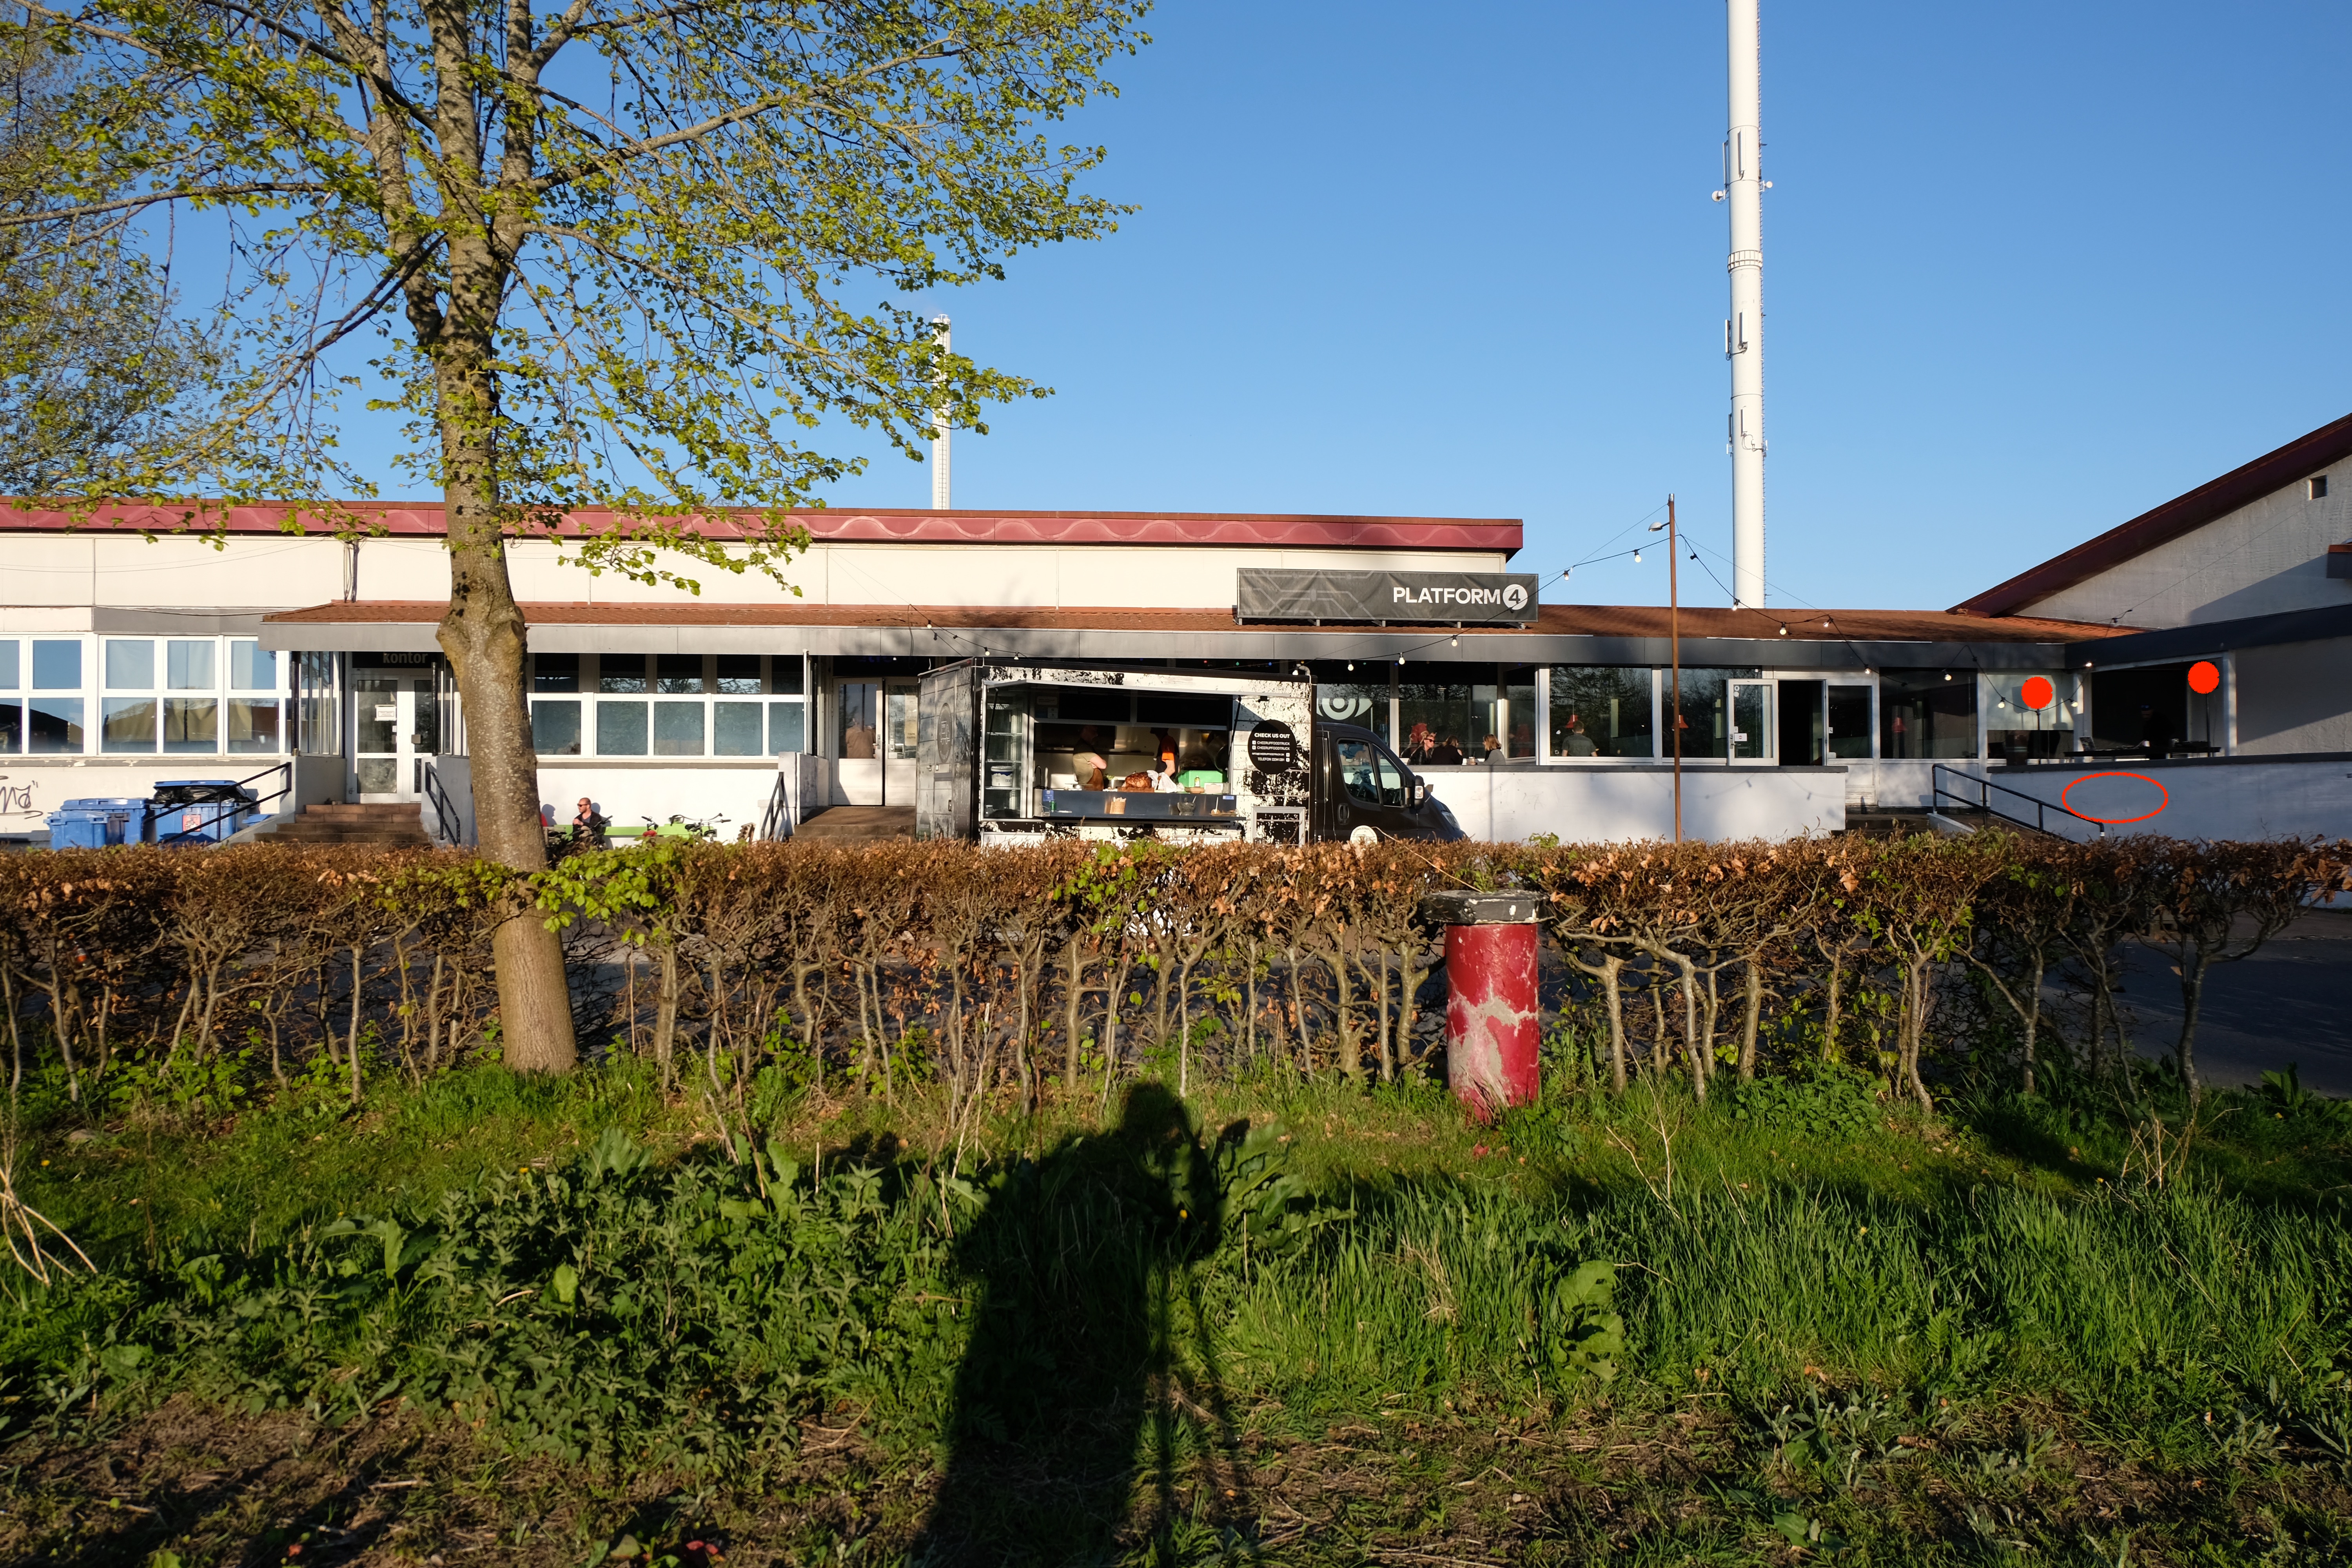
\includegraphics[width=1\textwidth]{Figures/P4day.jpg}
    \caption{Picture of the setup at the center point of the microphone array}
    \label{fig:Scenario4}
\end{figure}
\subsubsection{Results}
\begin{figure}[H]
    \centering
    \begin{subfigure}[b]{1\textwidth}
    \centering
    \includegraphics[width=1\textwidth]{Figures/P4_Day_6.png}
\end{subfigure}
\vskip \baselineskip
\begin{subfigure}[b]{1\textwidth}
    \centering
    \includegraphics[width=1\textwidth]{Figures/P4_Day_3.png}
\end{subfigure}
\caption{Figures depict from top-to-bottom Min SRP-PHAT with dynamic range of 6dB and 3dB(Zoomed)}
\label{Fig:P4Day}
\end{figure}
\subsection{Indoor concert}
Measurements were made of a concert happening indoors. The event took place at midnight, however the photo was taken during the day so that the overlay is easier to see.
\begin{figure}[H]
    \centering
    \begin{subfigure}[b]{1\textwidth}[H]
    \centering
    \includegraphics[width=1\textwidth]{Figures/P4Night6dB.png}
\end{subfigure}
\vskip \baselineskip
\begin{subfigure}[b]{1\textwidth}[H]
    \centering
    \includegraphics[width=1\textwidth]{Figures/P4Night3dB_Zoomed.png}
\end{subfigure}
\caption{Figures depict from top-to-bottom Min SRP-PHAT with dynamic range of 6dB and 3dB(Zoomed)}
\label{Fig:P4Night}
\end{figure}
\subsection{Roadside noise}
Cars passing through a crossing were measured in a close range ($2-10m$). A single loud motorcycle passing through was measured.
\subsubsection{General traffic}
\subsubsection{Loud motorcycle}
\subsection{Chalk mine}
A chalk mining machine was measured from a large distance ($500m$), with different microphone aperture sizes. The same measurement was then run closer ($100m$) and even closer ($90m$).
\subsection{Lookout large aperture}
\begin{figure}[H]
    \centering
    \includegraphics[width=1\textwidth]{Figures/ChalkFarFar.png}
    \caption{Localization results of the chalk mine from a far away lookout close to traffic noise}
    \label{fig:ChalkCLose}
\end{figure}
%\subsubsection{Lookout small aperture}
\subsubsection{Close to mine, far from edge}
\begin{figure}[H]
    \centering
    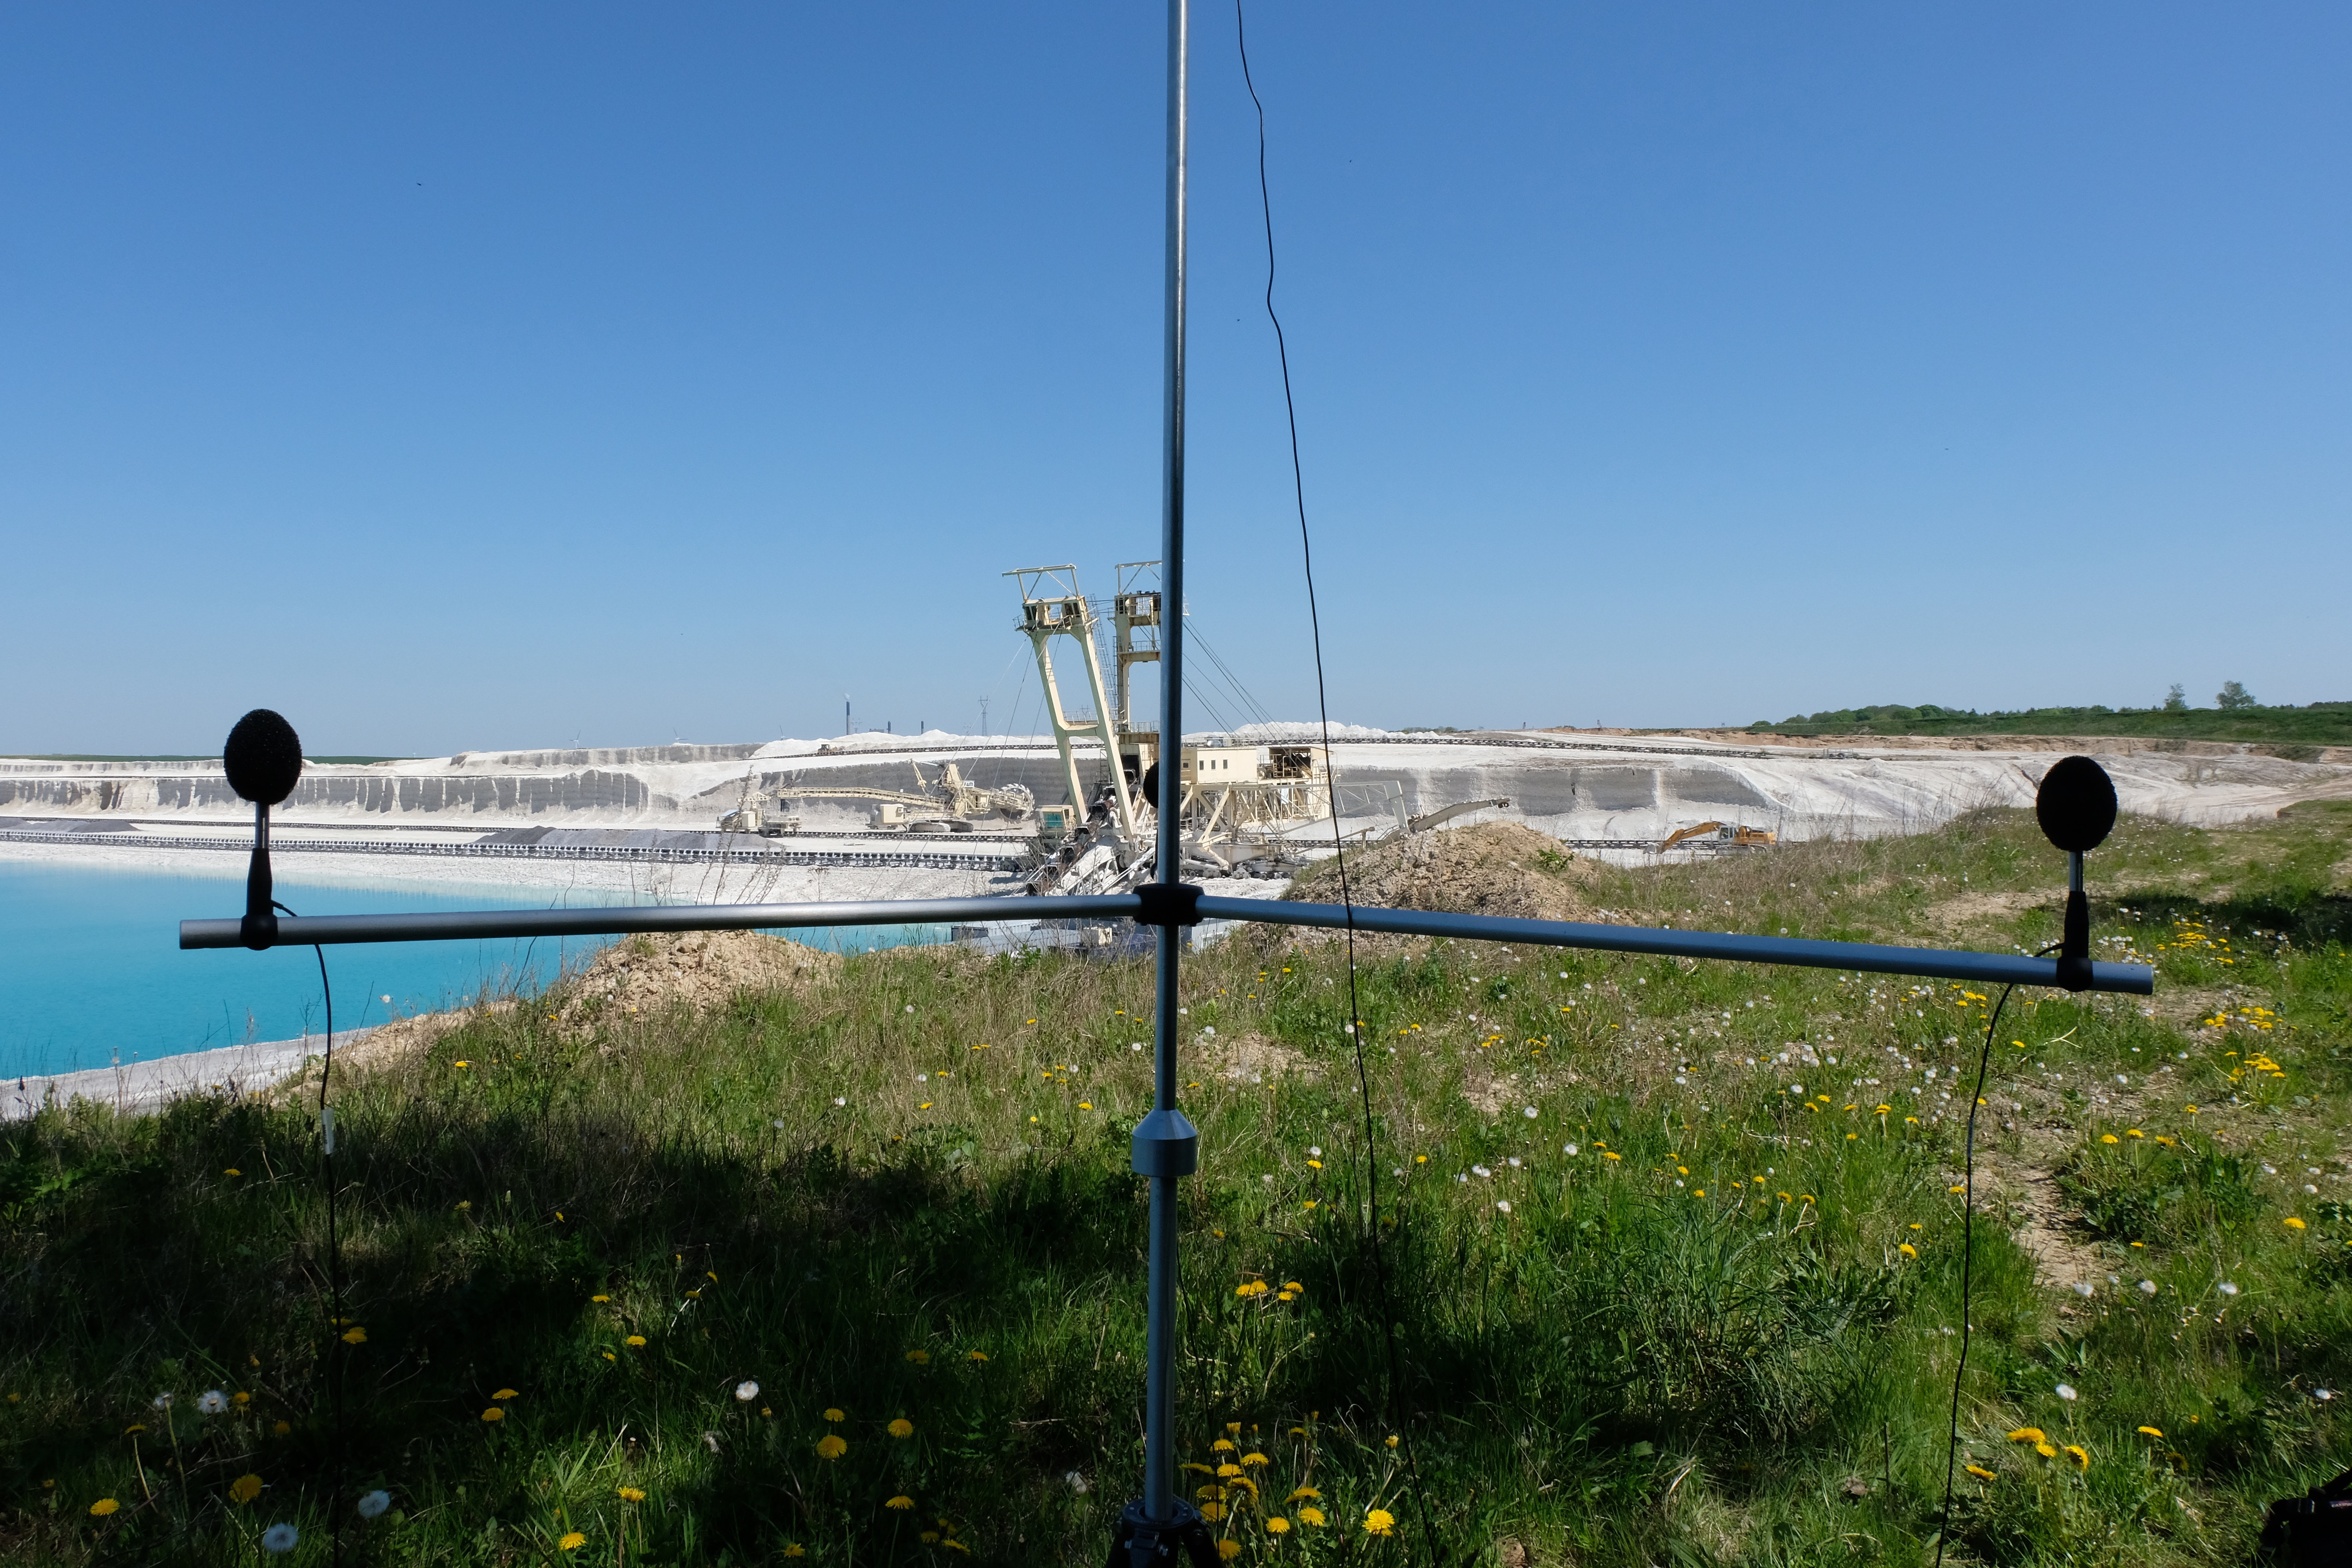
\includegraphics[width=1\textwidth]{Figures/ChalkFar.png}
    \caption{Localization results of the chalk mine far from the edge}
    \label{fig:ChalkCLose}
\end{figure}
\subsubsection{Close to mine, close to edge}
\begin{figure}[H]
    \centering
    \includegraphics[width=1\textwidth]{Figures/ChalkClose.png}
    \caption{Localization results of the chalk mine close to the edge}
    \label{fig:ChalkCLose}
\end{figure}

